\documentclass[conference]{IEEEtran}
\IEEEoverridecommandlockouts
% The preceding line is only needed to identify funding in the first footnote. If that is unneeded, please comment it out.
\usepackage{cite}
\usepackage{amsmath,amssymb,amsfonts}
\usepackage{algorithmic}
\usepackage{graphicx}
\usepackage{textcomp}
\usepackage{xcolor}
\usepackage{listings}
\usepackage{pgfplots}
\usepackage{float}
\pgfplotsset{compat=1.18}

\def\BibTeX{{\rm B\kern-.05em{\sc i\kern-.025em b}\kern-.08em
    T\kern-.1667em\lower.7ex\hbox{E}\kern-.125emX}}

\lstdefinestyle{mystyle}{
    basicstyle=\ttfamily\footnotesize,
    breakatwhitespace=false,         
    breaklines=true,                 
    captionpos=b,                    
    keepspaces=true,                                                       
    showspaces=false,                
    showstringspaces=false,
    showtabs=false,                  
    tabsize=2,
    frame=single,
    rulecolor=\color{black}
}

\lstset{style=mystyle}

\begin{document}

\title{Minimize Hand Displacement in a Song: Project 2 - Brute Force and Dynamic Programming}


\author{\IEEEauthorblockN{1\textsuperscript{st} Esteban Murillo}
\IEEEauthorblockA{\textit{Department of Computer Science} \\
\textit{Texas Tech University}\\
Lubbock, TX \\
estmuril@ttu.edu}
\and
\IEEEauthorblockN{2\textsuperscript{nd} Daniel Marin}
\IEEEauthorblockA{\textit{Department of Computer Science} \\
\textit{Texas Tech University}\\
Lubbock, TX \\
danimari@ttu.edu}
}

\maketitle

\begin{abstract}
This paper presents an algorithmic solution to optimize guitar chord transitions in musical sequences. We developed algorithms using both brute force and dynamic programming approaches to minimize left-hand displacement during chord changes. The system takes as input a sequence of chords in standard notation and a specification file containing multiple fingering positions for each chord. Our solution analyzes various possible chord positions and determines the optimal combination that minimizes the total hand movement throughout the song. The algorithms consider factors such as fret positions, string usage, and transitional distances between successive chord shapes. The results look to the difference and analyse the efficiency of the brute-force and dynamic programming approaches, based on the principal of demonstrating an effective method for reducing physical strain and improving playability in guitar performances through computational optimization.
\end{abstract}

\begin{IEEEkeywords}
dynamic programming, optimization algorithms, guitar chord transitions, musical computing, computational musicology, fingering optimization, performance automation
\end{IEEEkeywords}

\section{Introduction}
The optimization of musical performance through computational methods has become increasingly relevant in modern music technology. In this paper, we address a specific challenge in guitar playing: minimizing the left-hand movement during chord transitions.

When playing guitar, the positioning of the left hand on the fretboard significantly impacts both the physical effort required and the smoothness of the performance. A single chord can often be played in multiple positions on the fretboard, and the choice of these positions directly affects the distance the hand must travel when transitioning between chords. For instance, a C major chord can be played in several configurations, each requiring different finger placements and fret positions.

The challenge lies in determining the optimal sequence of chord positions that minimizes the total hand movement throughout an entire song. This optimization must consider various factors:
\begin{itemize}
    \item Multiple valid fingering positions for each chord
    \item The physical distance between successive chord positions
    \item The practical playability of the chosen sequences
    \item The specific requirements of open strings and unused strings in chord formations
\end{itemize}

To solve this problem, we developed two distinct algorithmic approaches. The first utilizes a brute force method, examining all possible combinations of chord positions to find the global optimum. The second employs dynamic programming techniques to efficiently compute the optimal solution by breaking down the problem into smaller subproblems and avoiding redundant calculations.

Our solution takes two inputs: a sequence of chords in standard musical notation (e.g., C, Am, Dm, G7) and a specification dictionary that details the various possible fingering positions for each chord. The dictionary uses a numerical representation system where each chord is defined by a sequence of numbers representing the fret positions for each string, with special notation for open strings (0) and unused strings.

\section{Methodology}
The Methodology of this project, is based on explaining the problem definition, each solution, and the comparisons between both. We also look to solve the following problem:
\newline
\indent``Polynizer has hired the excellent students of CS-3364 to create an algorithm that allows to find the optimal way to play the chords that the application infers, on the guitar. Specifically, we want to minimize the amount of movement made by the left hand. The algorithm takes as input the list of chords of a song in standard notation (e.g., C, Am, Dm, G7, and C) and a file specifying different ways to play each chord, and should print on the screen how to play each chord in order to minimize the total movement of the hand over the song.''\footnote[1]{Problem Definition stated in the project definition document by Arturo Camacho.}
\subsection{Problem Outline}
The algorithm we are looking to develop processes a song's chord sequence in standard notation (e.g., C, Am, Dm, G7) alongside a file detailing various fingerings for each chord, with the end goal of outputting the optimal sequence of chord fingerings that minimize the total hand movement throughout the song. Before understanding how the algorithm's solve this problem we first need to understand how solutions and inputs look like.
\newline 
\indent Both algorithms take in the same arguments. These arguments are as follows:
\begin{itemize}
    \item Chord List: that represents the sequence of n chords in a song. This is what the user writes in a `.txt' file. It has the expected format of a list/set of type:
    \( C = \{c_1, c_2, c_3, \dots, c_n\} \) where the \(c_i\) element in the list represents the \(i^{th}\) chord of the song.
    \item Chord Dict: is a helper dictionary that contains all possible fingerings of each chord instance; considering their offsets. Thus providing a mapping from chord to fingerings available. 
\end{itemize}
\indent These inputs remain consistent to both the brute-force search and the dynamic programming solution. Also, understanding the format of the inputs is required for comprehending the algorithms.
\newline
\indent Both algorithms return the same outputs, to answer (solve) the overall problem the user has. The outputs are:
\begin{itemize}
    \item Optimal Solution: this outputs represents the minimum hand displacement calculated for the list of chords being displaced. Results are in units of `frets displaced'.
    \item Optimal Vector: this output represents the vector \(\sigma = \{\sigma_1, \sigma_2, \sigma_2, \ldots, \sigma_n\} \) where the \(\sigma_i\) element in this vector represents the fingering to be played in \(i^{th}\) chord of the song. Where \( \sigma_i \in [0, K_i - 1] \), considering that \( K_i \) is the number of possible fingerings for the \(i^{th}\) chord.\footnote[2]{A \(c_i\) with 3 fingerings has possible values \(\sigma_i \in [0, 1, 2] \); where $0$ stands for the $1^{st}$ fingering in the .csv file, $1$ stands for the $2^{nd}$ fingering in the .csv file, and $2$ stands for the $3^{rd}$ fingering in the .csv file; a \(c_i\) with 2 fingerings has possible values \(\sigma_i \in [0, 1] \), and \(c_i\) with 1 fingering has possible values \(\sigma_i \in [0] \).}
    The \(\sigma\) represents the overall sequence of fingerings that minimize the overall hand displacement. 
    \item Optimal Sequence: this output represents the optimal vector as actual fingerings, it was used to debug the program. 
\end{itemize}
\indent The outputs represent the solution towards the problem that we look to solve. They provide the how and the value of the solution to the problem.
\newline
\indent Understanding the inputs and outputs of the black box (the algorithms), we need to look at some overlapping functions that are used to calculate displacement based on what the professor stated in the project definition document.
\subsection{Helper Functions}
The functions in this section look to provide a simple method to calculate the overall displacement between two chords. 
\begin{figure}[H]
\begin{lstlisting}[language=Python]
def calculate_average_fret(x):
    accum : int = 0
    frets : int = 0
    for fret in x:
        if fret is not None:
            accum += fret
            frets += 1
    return accum / frets if frets > 0 else 0.0
def calculate_movement_displacement(a, b):
    average_fret_a = calculate_average_fret(a)
    average_fret_b = calculate_average_fret(b)
    return (average_fret_a - average_fret_b)**2    
\end{lstlisting}
\caption{Uncommented functions in charge of calculating displacement of between fingerings, used in this project. Based, on program specifications in project definition document.}
\label{fig:DisplacementFunctions}
\end{figure}
The functions in Figure \ref{fig:DisplacementFunctions} are used to measure the displacement of the left hand on a guitar when transitioning between chord positions. The \lstinline|calculate_average_fret(x)| function calculates the centroid of a chord position by adding the fret numbers of all strings where the chord is fingering, and dividing it by the number of strings used by the fingering. For example: 
\[ \text{Centroid}_a  = \frac{0+2+2+2+0}{5} = 1.2 \] 
\[ \text{Centroid}_b = \frac{3+5+5+5+3}{5} = 4.2 \]
\indent Where \( \text{Centroid}_a \) represents chord A and \(\text{Centroid}_b \) represents chord C. 
\newline 
\indent The \lstinline|calculate_movement_displacement(a, b)| looks to calculate the displacement between two chords by calculating the following:
\[
\text{Displacement} = (\text{Centroid}_a + \text{Centroid}_b)^2
\]
\indent These function help the algorithm's minimize the processes being called, by centralizing them. With this understood, we may begin explaining the brute-force search algorithm that solves this problem.
\subsection{Brute-force Search}
Brute-force search is a straightforward and exhaustive problem-solving technique that systematically explores all possible solutions to a problem to identify the optimal one. It works by generating every potential candidate in the solution space, evaluating each against a given objective or constraint, and selecting the best match. While simple to implement and guaranteed to find the correct solution, brute-force search is often computationally expensive, as the number of possibilities grows exponentially with the size of the input. 
\subsubsection{Algorithm Design}
The algorithm designed for this project, regarding brute-force search, used exhaustive exploration of all possible sequences of fingerings from the chord list. 
There are various considerations, that should be looked at before evaluating the implementation of the algorithm: vector representation, its possible values, the space and its size.
\newline 
\noindent The vector has the same representation from the Problem Outline, that being: \[ \sigma = \{\sigma_1, \sigma_2, \sigma_3, \ldots, \sigma_n\} \] 
\indent Where \(\sigma_i \in [0, K_i - 1]\), and where \( K_i \) represents the number of possible fingerings of the $i^{th}$ chord in the song. If the resultant vector represents the solution, the vector space can be expressed as:
\[ S = \{0, \frac{\sum_{i=1}^{n}K_i - 1}{n} \}^{n} \]
\indent This setup of the vector space leads it to be upper bounded by \( S = \{0,1,2\}^{n} \), considering that the worst case scenario is a song composed of chords with $3$ fingerings available. The vector space size is:
\[ |S| = 3^{n} \].
\indent However, considering that there is a constraint where we should only allow chord fingerings that have base fret position of 7 or less, the space $S$ is further reduced to a subset $S'$ defined as:
\[ S' = \{\sigma \in S \mid \text{minimum fret position of \( F(C_{\sigma_i}) \)} \leq 7, \forall(i)\} \]
\indent This leads to a reduction in the vector space by an incalculable amount but in theory it should decrease or maintain the same.
\[ |S'| \leq |S| \]

\subsubsection{Asymptotic Time Complexity}
This algorithm has a time complexity of \(\Theta(3^{n})\) in the worst-case scenario, implying that this algorithm takes exponential time and is fairly inefficient for medium to large input sizes.  

\subsubsection{Code Implementation}
The brute force algorithm is implemented through several key components:

\begin{figure}[H]
\begin{lstlisting}[language=Python]
def minimum_movement_brute_force(chord_list, chord_dict):
    chord_fingerings = []
    for chord in chord_list:
        if chord in chord_dict:
            fingerings = []
            fingerings.append(chord_dict[chord]['Finger A'])
            if 'Finger B' in chord_dict[chord]:
                fingerings.append(chord_dict[chord]['Finger B'])
            if 'Finger C' in chord_dict[chord]:
                fingerings.append(chord_dict[chord]['Finger C'])
            chord_fingerings.append(fingerings)
\end{lstlisting}
\caption{First part of the brute force implementation: gathering possible fingerings}
\label{fig:BruteForceGather}
\end{figure}

The first part of the implementation (Figure \ref{fig:BruteForceGather}) focuses on gathering all possible fingerings for each chord in the sequence. The algorithm creates a list of available fingerings for each chord position, supporting up to three different fingering options (A, B, and C) per chord.

\begin{figure}[H]
\begin{lstlisting}[language=Python]
    for idx_combination in product(*[range(len(f)) for f in chord_fingerings]):
        sequence = [chord_fingerings[i][idx_combination[i]] 
                   for i in range(len(chord_list))]
        
        cost = total_movement_cost(sequence)
        
        if cost < min_cost:
            min_cost = cost
            min_cost_sequence = sequence
            min_cost_indices = list(idx_combination)
\end{lstlisting}
\caption{Core loop of the brute force implementation: evaluating all combinations}
\label{fig:BruteForceCore}
\end{figure}

The core of the algorithm (Figure \ref{fig:BruteForceCore}) systematically evaluates every possible combination of fingerings. It uses Python's \lstinline{itertools.product} to generate all possible combinations of fingering indices. For each combination:
\begin{itemize}
    \item Creates a sequence of actual fingerings using the current combination
    \item Calculates the total movement cost for this sequence
    \item Updates the optimal solution if a lower cost is found
\end{itemize}

\begin{figure}[H]
\begin{lstlisting}[language=Python]
def total_movement_cost(sequence):
    cost = 0
    for i in range(1, len(sequence)):
        cost += calculate_movement_displacement(sequence[i-1], sequence[i])
    return cost 
\end{lstlisting}
\caption{Helper function for calculating total movement cost}
\label{fig:BruteForceCost}
\end{figure}

The movement cost calculation (Figure \ref{fig:BruteForceCost}) iterates through the sequence of chords, summing up the displacement cost between consecutive chord positions. The first chord position serves as the starting point and doesn't contribute to the total cost.

The bounded version of the algorithm adds an additional constraint check:
\begin{lstlisting}[language=Python]
    if any(min(fret for fret in fingering if fret is not None) > 7 
           for fingering in sequence):
        continue
\end{lstlisting}

This optimization ensures that only fingerings within the first seven frets are considered, which both reduces the search space and produces more practical solutions for guitar players.

\subsection{Dynamic Programming}
Dynamic Programming (DP) is an algorithmic paradigm that solves complex problems by breaking them down into simpler subproblems. For our chord transition optimization, it is applicable because:
\begin{itemize}
    \item Each chord transition decision affects future transitions (overlapping subproblems)
    \item The optimal solution builds upon optimal solutions to smaller sequences (optimal substructure)
    \item Many chord transition patterns are evaluated multiple times (memoization opportunity)
\end{itemize}

\subsubsection{Oracle Definition}
The state space and transition function are defined as:

\begin{itemize}
    \item \(F(C_i)\): Set of valid fingerings for chord \(C_i\), where each fingering must have minimum fret position \(\leq 7\)
    \item Oracle[i][f]: Dictionary storing minimum cost to reach fingering f of chord i
    \item Solution[i][f]: Dictionary tracking previous fingering choices for solution reconstruction
\end{itemize}

A fingering f is considered valid if:
\[ \min(\{x \in f : x \neq \text{None}\}) \leq 7 \]

\subsubsection{Recurrence Relation}
The solution is built using:

\textbf{Base Case:}
\[ \text{Oracle}[0][f] = 0, \quad \forall f \in F(C_1) \text{ where f is valid} \]

\textbf{Recursive Step:}
For i from 1 to n-1:
\[ \text{Oracle}[i][f] = \min_{p \in F(C_{i-1})} \{\text{Oracle}[i-1][p] + \text{cost}(p, f)\} \]
where:
\begin{itemize}
    \item f is a valid fingering of chord i
    \item p is a valid fingering of chord i-1
    \item cost(p, f) is the squared displacement between fingerings
\end{itemize}

\textbf{Final Solution:}
\[ \min_{f \in F(C_n)} \text{Oracle}[n-1][f] \]

\subsubsection{Algorithm Implementation}
The implementation consists of four main components:

\begin{enumerate}
\item \textbf{Initialization}:
\begin{itemize}
    \item Collects valid fingerings for each chord from the chord dictionary
    \item Creates Oracle and Solution dictionaries for each chord position
    \item Sets base case costs for first chord's valid fingerings
\end{itemize}

\item \textbf{Oracle Construction}:
\begin{lstlisting}[language=Python]
# Fill the Oracle
for i in range(1, n):
    for f, fingering in enumerate(chord_fingerings[i]):
        if not is_valid_fingering(fingering):
            continue
        Oracle[i][f] = float('inf')
        for f_prev, prev_fingering in enumerate(chord_fingerings[i - 1]):
            if not is_valid_fingering(prev_fingering):
                continue
            cost = Oracle[i - 1][f_prev] + calculate_movement_displacement(prev_fingering, fingering)
            if cost < Oracle[i][f]:
                Oracle[i][f] = cost
                Solution[i][f] = f_prev
\end{lstlisting}

\item \textbf{Solution Reconstruction}:
\begin{itemize}
    \item Identifies minimum cost fingering for final chord
    \item Traces back through Solution dictionary to build optimal sequence
    \item Returns fingering indices and actual fingerings
\end{itemize}

\item \textbf{Cost Normalization}:
\[ \text{final\_cost} = \sqrt{\text{min\_cost}} \]
\end{enumerate}

\subsubsection{Time Complexity}
The algorithm achieves \(\Theta(n \times K^2)\) time complexity where:
\begin{itemize}
    \item n is the number of chords in the sequence
    \item K is the maximum number of valid fingerings for any chord
\end{itemize}

This is significantly more efficient than the brute force approach's \(\Theta(3^n)\) complexity, as it:
\begin{itemize}
    \item Eliminates redundant calculations through memoization
    \item Prunes invalid fingering combinations early
    \item Builds the solution incrementally using optimal substructure
\end{itemize}

\subsubsection{Code Implementation}
The dynamic programming algorithm is implemented through several key components:

\begin{enumerate}
\item \textbf{Helper Functions}:
\begin{lstlisting}[language=Python]
def is_valid_fingering(fingering):
    valid_frets = [fret for fret in fingering if fret is not None]
    if not valid_frets:
        return False
    return min(valid_frets) <= 7
\end{lstlisting}
This validation function ensures that:
\begin{itemize}
    \item Only considers frets that are actually used (not None)
    \item Returns False if no valid frets exist
    \item Enforces the constraint that minimum fret position must be \(\leq 7\)
\end{itemize}

\item \textbf{Fingering Collection}:
\begin{lstlisting}[language=Python]
chord_fingerings = []
for chord in chord_list:
    if chord in chord_dict:
        fingerings = []
        for key in ['Finger A', 'Finger B', 'Finger C']:
            if key in chord_dict[chord]:
                fingering = chord_dict[chord][key]
                fingerings.append(fingering)
\end{lstlisting}
This initialization phase:
\begin{itemize}
    \item Processes each chord in the input sequence
    \item Collects up to three possible fingerings (A, B, C) per chord
    \item Validates chord existence in the dictionary
\end{itemize}

\item \textbf{DP Table Construction}:
\begin{lstlisting}[language=Python]
n = len(chord_list)
Oracle = [{} for _ in range(n)]  # Each entry is a dictionary
Solution = [{} for _ in range(n)]  # Tracks previous indices

# Initialize base case
for f, fingering in enumerate(chord_fingerings[0]):
    if is_valid_fingering(fingering):
        Oracle[0][f] = 0
\end{lstlisting}
The initialization creates:
\begin{itemize}
    \item Two arrays of dictionaries for Oracle and Solution tracking
    \item Sets base case costs to 0 for valid first chord fingerings
\end{itemize}

\item \textbf{Core DP Algorithm}:
\begin{lstlisting}[language=Python]
for i in range(1, n):
    for f, fingering in enumerate(chord_fingerings[i]):
        if not is_valid_fingering(fingering):
            continue
        Oracle[i][f] = float('inf')
        for f_prev, prev_fingering in enumerate(chord_fingerings[i - 1]):
            if not is_valid_fingering(prev_fingering):
                continue
            cost = Oracle[i - 1][f_prev] + calculate_movement_displacement(
                prev_fingering, fingering)
            if cost < Oracle[i][f]:
                Oracle[i][f] = cost
                Solution[i][f] = f_prev
\end{lstlisting}
The main algorithm:
\begin{itemize}
    \item Iterates through each chord position
    \item For each valid current fingering
    \item Considers all valid previous fingerings
    \item Updates minimum cost and solution path
\end{itemize}

\item \textbf{Solution Reconstruction}:
\begin{lstlisting}[language=Python]
sequence = []
indexes = []
f = min_cost_index
for i in range(n - 1, -1, -1):
    sequence.append(chord_fingerings[i][f])
    indexes.append(f)
    f = Solution[i].get(f, None)
sequence.reverse()
indexes.reverse()
\end{lstlisting}
The reconstruction process:
\begin{itemize}
    \item Starts from the optimal final fingering
    \item Traces back through the Solution dictionary
    \item Builds both fingering sequence and index sequence
    \item Reverses sequences to get correct order
\end{itemize}
\end{enumerate}

The implementation uses dictionaries instead of traditional arrays to efficiently handle varying numbers of valid fingerings per chord. The final cost is normalized using square root to maintain consistency with the problem's distance metric.



\subsection{Greedy Approach}
A greedy algorithm was not implemented for this problem because a greedy approach cannot guarantee an optimal solution for chord sequence optimization. Here's why:

\begin{itemize}
    \item A greedy algorithm would make locally optimal choices at each step, selecting the chord fingering that minimizes movement from the current position
    \item However, these locally optimal choices do not necessarily lead to a globally optimal solution
    \item Consider this example:
    \begin{itemize}
        \item For a sequence "C-Am-G", a greedy approach might choose:
        \item The closest fingering of Am to the initial C chord position
        \item Then the closest G fingering to that Am position
        \item This could result in a larger total movement than choosing a slightly "worse" initial transition that enables a much better final transition
    \end{itemize}
    \item The problem requires considering the entire sequence of transitions to find the true optimal solution, which is why we implemented:
    \begin{itemize}
        \item Brute force approach: Guarantees optimality by checking all possibilities
        \item Dynamic programming approach: Efficiently finds the optimal solution by considering all possible combinations systematically
    \end{itemize}
\end{itemize}

Therefore, this project focuses on the brute force and dynamic programming solutions as they are capable of finding the globally optimal solution to the chord sequence optimization problem.

\section{Tests}
To evaluate the performance and effectiveness of both algorithms, we conducted tests using three musical pieces:

\begin{itemize}
    \item Luis Miguel Song
    \item Catch the Rainbow
\end{itemize}

\subsection{Test Setup}
Each algorithm was tested with different chord sequence lengths to analyze their scalability and performance characteristics:

\subsubsection{Brute Force Test Cases}
\begin{itemize}
    \item 1 chord sequence (first chord only)
    \item 5 chord sequence (first five chords)
    \item 10 chord sequence (first ten chords)
    \item 15 chord sequence (first fifteen chords)
    \item 20 chord sequence (first twenty chords)
\end{itemize}

\subsubsection{Dynamic Programming Test Cases}
\begin{itemize}
    \item 60 chord sequence (first sixty chords)
    \item 80 chord sequence (first eighty chords)
    \item 100 chord sequence (first one hundred chords)
    \item 120 chord sequence (first one hundred twenty chords)
\end{itemize}

\section{Results}
\subsection{Analysis - Luis Miguel Song}

\begin{table}[H]
\centering
\caption{Brute Force Execution Times - Luis Miguel Song}
\begin{tabular}{|c|c|}
\hline
\textbf{Number of Chords} & \textbf{Execution Time (seconds)} \\
\hline
1 & 0.000000 \\
5 & 0.001065 \\
10 & 0.021750 \\
15 & 0.555421 \\
20 & 65.967618 \\
\hline
\end{tabular}
\caption{Dynamic Programming Execution Times - Luis Miguel Song}
\begin{tabular}{|c|c|}
\hline
\textbf{Number of Chords} & \textbf{Execution Time (seconds)} \\
\hline
60 & 0.001003 \\
80 & 0.001509 \\
100 & 0.001005 \\
120 & 0.000977 \\
\hline
\end{tabular}
\label{tab:luismiguel_analysis_times}
\end{table}

\begin{figure}[H]
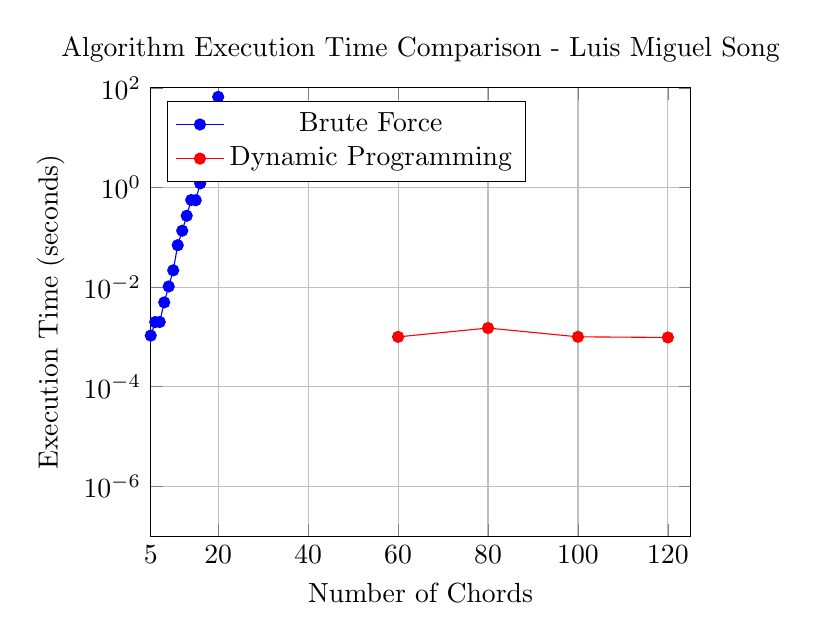
\begin{tikzpicture}
\begin{axis}[
    xlabel={Number of Chords},
    ylabel={Execution Time (seconds)},
    title={Algorithm Execution Time Comparison - Luis Miguel Song},
    grid=major,
    legend pos=north west,
    ymode=log,  % Using logarithmic scale for better visualization
    xtick={5,20,40,60,80,100,120},
    xmin=5,
    xmax=125,
    ymin=0.0000001,
    ymax=100,
    legend entries={Brute Force, Dynamic Programming}
]
\addplot[color=blue,mark=*] coordinates {
    (5,0.001065)
    (6,0.001991)
    (7,0.001997)
    (8,0.004937)
    (9,0.010312)
    (10,0.021750)
    (11,0.069454)
    (12,0.135738)
    (13,0.270776)
    (14,0.561291)
    (15,0.555421)
    (16,1.209936)
    (17,3.419934)
    (18,6.955780)
    (19,22.249811)
    (20,65.967618)
};
\addplot[color=red,mark=*] coordinates {
    (60,0.001003)
    (80,0.001509)
    (100,0.001005)
    (120,0.000977)
};
\end{axis}
\end{tikzpicture}
\caption{Exponential growth of execution time with increasing chord sequence length}
\label{fig:luismiguel_bf_graph}
\end{figure}

\textbf{Analysis of Results:}
The execution time results demonstrate the exponential nature of the brute force algorithm (Blue line):

\begin{itemize}
    \item \textbf{Single Chord (1):} Negligible execution time (0.000000s), as only one fingering combination needs to be evaluated
    \item \textbf{Five Chords (5):} Slight increase in execution time (0.0.001065s), still maintaining efficient performance
    \item \textbf{Ten Chords (10):} Notable jump to 0.021750s, showing the beginning of exponential growth
    \item \textbf{Fifteen Chords (15):} Significant increase to 0.555421s, approximately 22 times slower than the 10-chord sequence
    \item \textbf{Twenty Chords (20):} Execution time of 65.967618s, demonstrating the impracticality of brute force for longer sequences
\end{itemize}

The graph clearly shows the exponential growth pattern, with execution time increasing dramatically as the number of chords increases. This aligns with the algorithm's theoretical time complexity of \(\Theta(3^n)\), where n is the number of chords. The steep curve between 10 and 15 chords particularly highlights why brute force becomes impractical for longer sequences.

In contrast, the dynamic programming solution (Red line) demonstrates remarkably consistent performance:

\begin{itemize}
    \item \textbf{Sixty Chords (60):} Execution time of 0.001003s
    \item \textbf{Eighty Chords (80):} Slight increase to 0.001509s
    \item \textbf{One Hundred Chords (100):} Maintained efficiency at 0.001005s
    \item \textbf{One Hundred Twenty Chords (120):} Consistent performance at 0.000977s
\end{itemize}

The dynamic programming results showcase several key advantages:

\begin{itemize}
    \item \textbf{Scalability:} The algorithm maintains near-constant execution times even as the input size triples from 40 to 120 chords
    \item \textbf{Efficiency:} Processing 120 chords takes approximately the same time as the brute force approach needs for just 5 chords
    \item \textbf{Consistency:} The slight variations in execution time (between 0.000977s and 0.001509s) demonstrate stable performance regardless of input size
    \item \textbf{Practical Applicability:} The algorithm's ability to handle large chord sequences in milliseconds makes it suitable for real-world applications
\end{itemize}

These results validate the theoretical time complexity of \(\Theta(n \times K^2)\) for the dynamic programming solution, where n is the number of chords and K is the maximum number of fingerings per chord. The nearly flat line in the graph demonstrates how this polynomial-time complexity translates to practical performance benefits, especially when compared to the exponential growth of the brute force approach.

\subsection{Analysis - Halsey Song}

\begin{table}[H]
\centering
\caption{Brute Force Execution Times - Halsey Song}
\begin{tabular}{|c|c|}
\hline
\textbf{Number of Chords} & \textbf{Execution Time (seconds)} \\
\hline
5 & 0.001006 \\
10 & 0.006088 \\
15 & 0.236356 \\
20 & 19.808614 \\
\hline
\end{tabular}
\caption{Dynamic Programming Execution Times - Halsey Song}
\begin{tabular}{|c|c|}
\hline
\textbf{Number of Chords} & \textbf{Execution Time (seconds)} \\
\hline
60 & 0.001021 \\
80 & 0.000958 \\
100 & 0.001006 \\
120 & 0.001001 \\
\hline
\end{tabular}
\label{tab:halsey_analysis_times}
\end{table}

\begin{figure}[H]
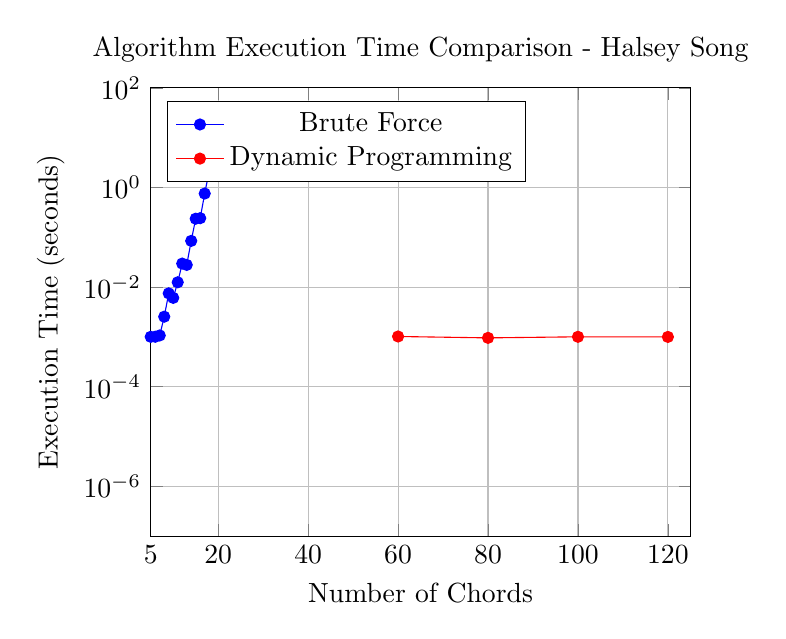
\begin{tikzpicture}
\begin{axis}[
    xlabel={Number of Chords},
    ylabel={Execution Time (seconds)},
    title={Algorithm Execution Time Comparison - Halsey Song},
    grid=major,
    legend pos=north west,
    ymode=log,
    xtick={5,20,40,60,80,100,120},
    xmin=5,
    xmax=125,
    ymin=0.0000001,
    ymax=100,
    legend entries={Brute Force, Dynamic Programming}
]
\addplot[color=blue,mark=*] coordinates {
    (5,0.001006)
    (6,0.001009)
    (7,0.001072)
    (8,0.002550)
    (9,0.007499)
    (10,0.006088)
    (11,0.012514)
    (12,0.029697)
    (13,0.027930)
    (14,0.084792)
    (15,0.236356)
    (16,0.242440)
    (17,0.756384)
    (18,2.156566)
    (19,6.638306)
    (20,19.808614)
};
\addplot[color=red,mark=*] coordinates {
    (60,0.001021)
    (80,0.000958)
    (100,0.001006)
    (120,0.001001)
};
\end{axis}
\end{tikzpicture}
\caption{Execution time comparison for Halsey song analysis}
\label{fig:halsey_bf_graph}
\end{figure}

\textbf{Analysis of Results:}
The execution time results for the Halsey song demonstrate similar patterns to the previous analysis:

\begin{itemize}
    \item \textbf{Brute Force Performance:}
    \begin{itemize}
        \item \textbf{Five Chords:} Very efficient at 0.001006s
        \item \textbf{Ten Chords:} Modest increase to 0.006088s
        \item \textbf{Fifteen Chords:} Significant jump to 0.236356s
        \item \textbf{Twenty Chords:} Major increase to 19.808614s
    \end{itemize}
    
    \item \textbf{Dynamic Programming Performance:}
    \begin{itemize}
        \item Consistently efficient performance across all test cases
        \item Execution times remain stable between 0.000958s and 0.001021s
        \item No significant performance degradation even at 120 chords
    \end{itemize}
\end{itemize}

The results show that while the brute force approach still exhibits exponential growth, it performs somewhat better on this song compared to the Luis Miguel analysis. This could be due to:

\begin{itemize}
    \item Different chord complexity in the sequence
    \item Varying number of possible fingerings per chord
    \item More efficient pruning of invalid combinations
\end{itemize}

The dynamic programming solution maintains its superior performance characteristics, processing the entire 120-chord sequence in approximately the same time that the brute force approach needs for 5-6 chords. This further validates the algorithm's practical applicability for real-world use cases.

\section{Conclusion}


% \begin{thebibliography}{00}

% \end{thebibliography}

\end{document}